\documentclass[review]{elsarticle}

\usepackage{hyperref}
\usepackage{verbatim}
\usepackage{amsmath}
\usepackage{amssymb}
\usepackage{slashed}
\usepackage{xcolor}
\usepackage{booktabs}

\usepackage{minted}  % syntax highlighting
\definecolor{bg}{rgb}{0.94,0.94,0.94}
\usemintedstyle{pastie}
\newcommand{\mil}[1]{\mintinline{python}{#1}}

\journal{Computer Physics Communications}

% Numbered without titles
\bibliographystyle{model1a-num-names}

% `Elsevier LaTeX' style
%\bibliographystyle{elsarticle-num}

\newcommand{\us}[1]{{~\mathrm{#1}}}
\renewcommand\u[1]{{\mathrm{#1}}}
\renewcommand\L{\mathcal{L}}
\renewcommand\d{\partial}

% hazma commands
% \newcommand{\hazma}{\texttt{hazma}}
% \newcommand{\theory}{\texttt{theory}}
% \newcommand{\sm}{\texttt{scalar\_mediator}}
% \newcommand{\vm}{\texttt{vector\_mediator}}
\newcommand{\hazma}{\mil{hazma}}
\newcommand{\theory}{\mil{theory}}
\newcommand{\sm}{\mil{scalar_mediator}}
\newcommand{\vm}{\mil{vector_mediator}}
\newcommand{\svann}{\langle \sigma v \range_{\bar{\chi} \chi}}


\begin{document}




\begin{frontmatter}

	\title{Hazma\tnoteref{mytitlenote}}
	\tnotetext[mytitlenote]{Code and tutorials available at \href{https://github.com/LoganAMorrison/Hazma}{github.com/LoganAMorrison/Hazma}.}

	\author[grappa,ucsc,scipp]{Adam Coogan}
	\ead{a.m.coogan@uva.nl}

	\author[ucsc,scipp]{Logan A. Morrison}
	\ead{loanmorr@ucsc.edu}

	\address[grappa]{GRAPPA, Institute of Physics, University of Amsterdam, 1098 XH Amsterdam, The Netherlands}
	\address[ucsc]{Department of Physics, 1156 High St., University of California Santa Cruz, Santa Cruz, CA 95064, USA}
	\address[scipp]{Santa Cruz Institute for Particle Physics, 1156 High St., Santa Cruz, CA 95064, USA}

	\begin{abstract}
		Hazma does many wonderful things.
	\end{abstract}

	\begin{keyword}
		Dark matter \sep indirect detection
	\end{keyword}

\end{frontmatter}

\section{Introduction}

Hazma is great.

\paragraph{Notation/units} Unless otherwise noted, the units used throughout \hazma\ are
\begin{itemize}
    \item Masses: MeV
    \item Decay widths: MeV
    \item Cross sections: $\u{cm}^3 / \u{s}$
    \item The \mil{numpy} package is referred to in some of the code snippets.
    \item We have sometimes rounded or formatted the output from \mil{hazma} to make the code snippets more readable.
\end{itemize}

\section{Installation and Package Structure}%
\label{sec:installation}

\subsection{Installation}

Before installing \texttt{hazma}, the user needs to have a few of well-established packages : cython, scipy, numpy, and scikit-image. Theses are easily installed by using PyPi. If the user has PyPi installed on their system, then these packages can be installed using
\begin{verbatim}
	pip install cython, scipy, numpy, scikit-image, matplotlib
\end{verbatim}
Hazma can be installed in the same way, using:
\begin{verbatim}
	pip install hazma
\end{verbatim}
This will download a tarball from the PyPi repository, compile all the c-code and install \texttt{hazma} on the system. Alternatively, the user can install \texttt{hazma} by downloading the package from \url{https://github.com/LoganAMorrison/Hazma.git}. Once downloaded, navigate to the package directory using the command line and run either
\begin{verbatim}
	pip install .
\end{verbatim}
or
\begin{verbatim}
	python setup.py install
\end{verbatim}


Note that since \texttt{hazma} makes extensive usage of the package cython, the user will need to have a c-compiler installed on their system. For more information, see the cython installation guide: \url{https://cython.readthedocs.io/en/latest/src/quickstart/install.html}




\section{Overview: The \texttt{theory} Class}%
\label{sec:overview_the_theory_class}

{\color{red} Should we have boxes for different functions and constructors specifying type signatures? Should that be left for the actual docs in the code? Seems like it, based on other publications in this journal?}

Instances of the \theory\ class represent dark matter models, and are the main objects used to perform analyses in Hazma. Two \theory\s, each containing a DM and mediator particle, come built into \hazma. The Lagrangians defining these theories and the domains of validity are described in the following subsection. \theory\ possesses methods to compute quantities such as DM annihilation cross sections, gamma ray spectra and constraints, and CMB constraints. This section catalogues the definitions of these quantities used by \hazma\ along with minimal examples of how to use the associated methods.

\subsection{Built-in Theories}%
\label{sub:built_in_theories}

{\color{red} Present Lagrangians for scalar and vector models. Link to github with FR and FC calculations.}

Each of the models that ship with \hazma\ contain two BSM particles:
\begin{itemize}
    \item A dark matter particle;
    \item A mediator $M$ that interacts with the DM as well as Standard Model particles.
\end{itemize}
The Lagrangians can be expressed as
\begin{align}
    \L &= \L_\u{SM} + \L_\u{DM} + \L_\u{M} + \L_{\u{Int}(M)},
\end{align}
which consists of the SM Lagrangian, the free Lagrangians for the mediator and DM, and the mediator's interactions with the DM and SM fields. Both the dark matter and the mediator are taken to be uncharged under the Standard Model gauge group. The Lagrangian is defined in terms of the microscopic degrees of freedom of the Standard Model (quarks, leptons and gauge bosons). However, at the energy scale of interest for self-annihilations of nonrelativistic MeV dark matter, quarks and gluons are not the corrent strongly-interacting degrees of freedom. Instead, the microscopic Lagrangian must be matched onto the effective Lagrangian for pions and other mesons using the techniques of chiral perturbation theory (chPT). The models currently implemented in \hazma\ utilize leading-order chPT. 

\begin{figure}
    \centering
    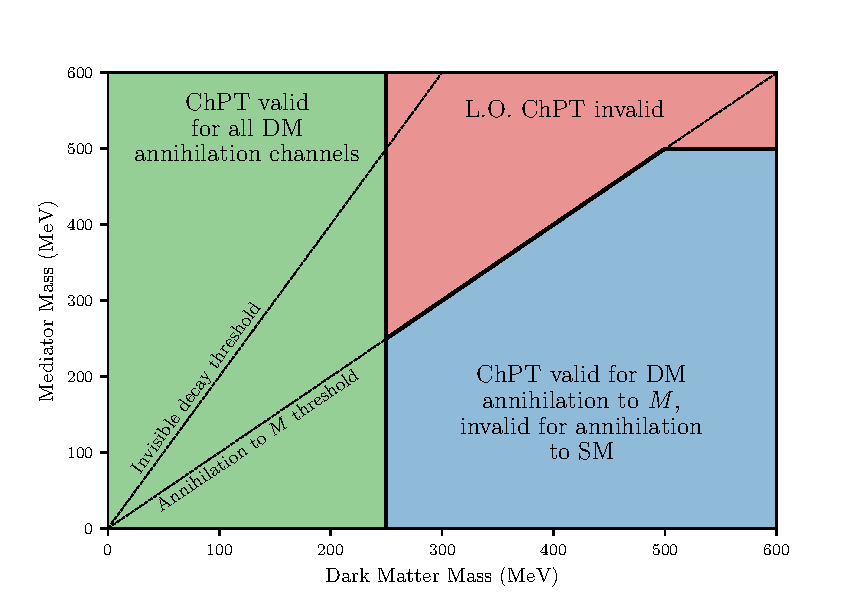
\includegraphics[width=\linewidth]{figures/med_and_dm_mass_phase_diagram.pdf}
    \caption{Values of the DM mass $m_\u{DM}$ and mediator mass $m_M$ for which the leading-order chiral perturbation theory calculations used to implement the models built into \hazma\ can be trusted.}
    \label{fig:chpt_validity}
\end{figure}

As with an effective field theory (EFT), chPT has a limited range of validity. Observables in chPT are computed in terms of an expansion in a small parameter, the meson momentum $p$ divided by the mass scale $\Lambda_\u{ChPT} \sim 4 \pi f_\pi \sim 1\us{GeV}$, where $f_\pi$ is the pion decay constant. As $p^2 \to \Lambda_\u{ChPT}$, higher-order Feynman diagrams in the chPT expansion provide contributions to observables comparable to leading order ones. This suggests that leading-order chPT cannot be trusted for computing dark matter self-annihilation cross sections when $m_\u{DM} \gtrsim 500\us{GeV}$. In fact, the convergence of the chPT expansion is disrupted at a lower mass scale by the lowest-lying hadronic resonances, the $\rho$ ($m_\rho = 770\us{GeV}$) and the $f_0(500)$ ($m_{f_0(500)} \sim 450\us{MeV}$). Figure~\ref{fig:chpt_validity} illustrates the resulting regions where the leading-order chPT calculations can and cannot be trusted in the $(m_\u{DM}, m_\u{mediator})$ plane. An important consequence is that annihilation into kaons and heavier mesons can be ignored since that would require DM masses far above the chPT range of validity. This is important to keep in mind when using the models provided with \hazma.\footnote{Of course, user-defined models (see Section~\ref{sec:advanced_usage}) need not use leading-order chPT.}

While the preceding discussion applies irrespective of the mediator and DM spin and quantum numbers, the rest of this subsection specializes to the two models that come with \hazma: \sm, which contains a real scalar mediator $S$ and \vm, where the mediator is a vector $V$.
 In both cases the DM is taken to be a Dirac fermion, so that
\begin{align}
    \L &= \bar{\chi} (i \slashed \d - m_\chi) \chi.
\end{align}
The rest of this subsection presents $\L_{\u{Int}(S)}$ and $\L_{\u{Int}(V)}$ at the level of quarks and gluons as well as the Lagrangians obtained by performing the chPT matching. Snippets are provided to demonstrate how to construct each \theory\ and change its parameters. The interaction Lagrangians, matching procedure and a brief overview of the chiral Lagrangian are explained in detail in a companion paper~\cite{matching_paper}.

\subsubsection{\sm}

The free Lagrangian for a real scalar is
\begin{align}
    \L_S &= \frac{1}{2} (\d_\mu S) (\d^\mu S) - \frac{1}{2} m_S^2 S^2,
\end{align}
where $m_S$ is the scalar's mass. The interactions with the light fundamental SM degrees of freedom
\begin{align}
    \L_{\u{Int}(S)} &= -S \left( g_{S\chi} + g_{Sf} \sum_f \frac{y_f}{\sqrt{2}} \bar{f} f \right)\\
                    &\hspace{2cm} + \frac{S}{\Lambda} \left( g_{SF} \frac{\alpha_\u{EM}}{4\pi} F_{\mu\nu} F^{\mu\nu} + g_{SG} \frac{\alpha_s}{4\pi} G_{\mu\nu}^a G^{a \mu\nu} \right).
\end{align}
The sum runs over fermions with mass below the GeV scale ($f = e, \mu, u, d, s$). Note that the coupling $g_{Sf}$ is outside the sum. The Yukawas are defined to be $y_f = \sqrt{2} m_f / v_h$, with the Higgs vacuum expectation value (vev) defined as $v_h = 246\us{GeV}$. The parameter $\Lambda$ is the mass scale at which $S$ acquires (non-renormalizable) interactions with the photon and gluon.

After performing the matching onto the chiral Lagrangian and expanding to leading order in the pion fields, the resulting interaction Lagrangian is
\begin{align}
    \L_{\mathrm{Int}(S)} &= \frac{2 g_{SG}}{9 \Lambda} S \left[ (\d_\mu \pi^0) (\d^\mu \pi^0) + 2 (\d_\mu \pi^+) (\d^\mu \pi^-) \right]\\
                         &\hspace{1cm} + \frac{4 i e g_{SG}}{9 \Lambda} S A^\mu \left[ \pi^- (\d_\mu \pi^+) - \pi^+ (\d_\mu \pi^-) \right]\\
                         &\hspace{1cm} - \frac{B (m_u + m_d)}{6} \left( \frac{3 g_{Sf}}{v_h} + \frac{2 g_{SG}}{3 \Lambda} \right) S \left[ (\pi^0)^2 + 2 \pi^+ \pi^- \right]\\
                         &\hspace{1cm} + \frac{B (m_u + m_d) g_{SG}}{81 \Lambda} \left( \frac{2 g_{SG}}{\Lambda} - \frac{9 g_{Sf}}{v_h} \right) S^2 \left[ (\pi^0)^2 + 2 \pi^+ \pi^- \right]\\
                         &\hspace{1cm} + \frac{4 e^2 g_{SG}}{9\Lambda} S \pi^+ \pi^- A_\mu A^\mu\\
                         &\hspace{1cm} - g_{S \chi} S \bar{\chi} \chi - g_{Sf} S \sum_{\ell=e,\mu} \frac{y_\ell}{\sqrt{2}} \bar{\ell} \ell + \frac{\alpha_s}{4\pi \Lambda} g_{SG} S G_{\mu\nu}^a G^{a \mu\nu}.
\end{align}

The parameters for the scalar model are attributes of the \sm\ class. Their names in \hazma\ are
\begin{align*}
    (m_\chi, m_S, g_{S\chi}, g_{Sf}, g_{SG}, g_{SF}, \Lambda) \leftrightarrow (\mathtt{mx}, \mathtt{ms}, \mathtt{gsxx}, \mathtt{gsff}, \mathtt{gsGG}, \mathtt{gsFF}, \mathtt{lam}).
\end{align*}
The following snippet shows how to instantiate \sm, change the value of a parameter, and print its new value:
\begin{minted}[bgcolor=bg]{python}
>>> from hazma.scalar_mediator import ScalarMediator
>>> sm = ScalarMediator(mx=150., ms=1e3, gsxx=1., gsff=0.1,
...                     gsGG=0.1, gsFF=0.1, lam=2e5)
>>> print(sm.gsff)
0.1
>>> sm.gsff = 0.5
>>> print(sm.gsff)
0.5
\end{minted}

{\color{red} Talk about Higgs portal and heavy fermion subclasses!}

\subsubsection{\vm}

For the vector mediator the free part of the Lagrangian is
\begin{align}
    \L_V &= -\frac{1}{4} V_{\mu\nu} V^{\mu\nu} + \frac{1}{2} m_V^2 V_\mu V^\mu,
\end{align}
where $m_V$ is the mass of the vector. The interactions considered are
\begin{align}
    \L_{\u{Int}(V)} &= V_\mu \left( g_{V\chi} \bar{\chi} \gamma^\mu \chi + \sum_f g_{Vf} \bar{f} \gamma^\mu f \right) - \frac{\epsilon}{2} V^{\mu\nu} F_{\mu\nu}.
\end{align}
The sum again runs over the light fermions ($f = e, \mu, u, d, s$), and $V$ may have different couplings to each of these. The last term is a kinetic mixing between the photon and $V$, which can be eliminated by transforming the photon $A_\mu \to A_\mu - \epsilon V_\mu$. Upon this field redefinition $V$ acquires an $\epsilon$-suppressed interaction with the SM fermions, which is captured by changing the fermion couplings
\begin{align}
    g_{Vf} \to g_{Vf} - \epsilon e Q_f,
\end{align}
where $Q_f$ is the electric charge of the fermion $f$ and $e > 0$ is the electron's charge.

Matching onto the chiral Lagrangian and isolating the terms contributing at leading order to the quantities computed in \hazma\ gives
\begin{align}
    \L_{\mathrm{Int}(V)} &= -i (g_{Vu} - g_{Vd}) V^\mu \left( \pi^+ \d_\mu \pi^- - \pi^- \d_\mu \pi^+ \right)\\
                         &\hspace{1cm} + ( g_{Vu} - g_{Vd} )^2 V_\mu V^\mu \pi^+ \pi^-\\
                         &\hspace{1cm} + 2 e (Q_u - Q_d) (g_{Vu} - g_{Vd}) A_\mu V^\mu \pi^+ \pi^-\\
                         &\hspace{1cm} + \frac{1}{8\pi^2 f_\pi} \epsilon^{\mu\nu\rho\sigma} (\d_\mu \pi^0)\\
                         &\hspace{2cm} \times \left\{ e (2 g_{Vu} + g_{Vd}) \left[ (\d_\nu A_\rho) V_\sigma + (\d_\nu V_\rho) A_\sigma \right] \right.\\
                         &\hspace{4cm} \left. + 3 (g_{Vu}^2 - g_{Vd}^2) (\d_\nu V_\rho) V_\sigma \right\}.
\end{align} 

The correspondence between the microscopic parameters for the vector model and attributes of the base \vm\ class is\footnote{Note that $\mil{gvss}$ is not currently used since \vm\ is based on leading-order chPT.}
\begin{align*}
    &(m_\chi, m_V, g_{V\chi}, g_{Vu}, g_{Vd}, g_{Vs}, g_{Ve}, g_{V\mu})\\
    &\hspace{1cm} \leftrightarrow (\mil{mx}, \mil{mv}, \mil{gvxx}, \mil{gvuu}, \mil{gvdd}, \mil{gvss}, \mil{gvee}, \mil{gvmumu}).
\end{align*}
The following snippet shows how to instantiate and alter the parameter values for \vm:
\begin{minted}[bgcolor=bg]{python}
>>> from hazma.vector_mediator import VectorMediator
>>> vm = VectorMediator(mx=150., mv=1e3, gvxx=1., gvuu=0.1,
...                     gvdd=0.2, gvss=0.3, gvee=0.4,
...                     gvmumu=0.5)
>>> print(vm.gvee)
0.4
>>> print(vm.gvuu)
0.1
>>> vm.gvuu = 0.05
>>> print(vm.gvuu)
0.05
\end{minted}

For convenience, a subclass called \mil{KineticMixing} is also provided to handle the important case where $V$ couples to the SM purely through the kinetic mixing term ($\epsilon \neq 0$, $g_{Vf} = 0$ for all $f$). The parameters for this subclass are
\begin{align*}
    (m_\chi, m_V, g_{V\chi}, \epsilon) \leftrightarrow (\mil{mx}, \mil{mv}, \mil{gvxx}, \mil{eps}).
\end{align*}
While the underlying parameters \mil{gvuu}, \dots, \mil{gvmumu} can be accessed by instances of \mil{KineticMixing}, they cannot be set directly since they are fully determined by \mil{eps}:
\begin{minted}[bgcolor=bg]{python}
>>> from hazma.vector_mediator import KineticMixing
>>> km = KineticMixing(mx=150., mv=1e3, gvxx=1., eps=0.1)
>>> km.eps
0.1
>>> km.gvuu
-0.020187846690459792  # = -0.1 * 2/3 * sqrt(4 pi / 137)
>>> km.gvuu = 0.1
AttributeError: Cannot set gvuu
\end{minted}

\subsection{Cross section, decay widths and branching fractions}

Instances of \mil{theory} provide the following four methods for computing particle physics quantities.

\subsubsection{\mil{Theory.list_annihilation_final_states()}}

Lists the final states into which the DM can potentially annihilate. These are based on the terms appearing in $\L_{\u{Int}(M)}$. Note that the actual branching fractions into a given final state may be zero if the relevant couplings are zero or the center of mass energy for the annihilation is smaller than the sum of the final state particles' masses. 
\begin{minted}[bgcolor=bg]{python}
>>> ScalarMediator.list_annihilation_final_states()
['mu mu', 'e e', 'g g', 'pi0 pi0', 'pi pi', 's s']
>>> VectorMediator.list_annihilation_final_states()
['mu mu', 'e e', 'pi pi', 'pi0 g', 'v v']
\end{minted}
{\color{red} This is not quite right. For example, it excludes the final states $e^+ e^- \gamma$, $S \pi^0 \pi^0$, $\pi^+ \pi^- \gamma \gamma$ for the scalar and $V \pi^0$ for the vector. While that's fine since those final states are so suppressed, the wording here needs to be precise.}

\subsubsection{\mil{Theory.annihilation_cross_sections(e_cm)}}

For an instance \mil{th} of \mil{theory} and a center of mass energy \mil{e_cm}, this returns a \mil{dict} whose keys are the elements of \mil{th.list_annihilation_final_states()} and \mil{'total'} and whose values are the corresponding cross sections for annihilating into those states. In the theories included with \hazma, the propagators used for the mediators take into account their widths.

In the following example, the DM is lighter than the mediator, but the center of mass energy is large enough to permit annihilations into the mediator:
\begin{minted}[bgcolor=bg]{python}
>>> sm = ScalarMediator(mx=180., ms=190., gsxx=1., gsff=0.1,
...                     gsGG=0.1, gsFF=0.1, lam=2e5)
>>> xsecs = sm.annihilation_cross_sections(400.)
>>> print(xsecs)
{'g g': 5.668702951121324e-32,
 'e e': 4.525214520210817e-32,
 'pi0 pi0': 1.8542010286144253e-27,
 'total': 4.1600065791804136e-18,
 's s': 4.160006572615015e-18,
 'mu mu': 1.1842156064646993e-27,
 'pi pi': 3.526880321768581e-27}
\end{minted}

\subsubsection{\mil{Theory.annihilation_branching_fractions(e_cm)}} 

For an instance \mil{th} of \mil{theory} and a center of mass energy \mil{e_cm}, this returns a \mil{dict} whose keys are the elements of \mil{th.list_annihilation_final_states()} and whose values are the corresponding branching fractions for annihilating into those states.
\begin{minted}[bgcolor=bg]{python}
>>> km = KineticMixing(mx=170., mv=1e3, gvxx=1., eps=0.2)
>>> bfs = km.annihilation_branching_fractions(400.)
>>> print(bfs)
{'pi0 g': 1.5585058782195258e-05,
 'e e': 0.4855695299567697,
 'mu mu': 0.4698109970123726,
 'v v': 0.0,
 'pi pi': 0.04460388797207543}
\end{minted}

\subsubsection{\mil{Theory.partial_widths()}}

Returns a \mil{dict} whose keys are states into which the mediator can decay and whose values are the corresponding decay widths.
\begin{minted}[bgcolor=bg]{python}
>>> vm = VectorMediator(mx=100, mv=300, gvxx=0.5, gvuu=0.3,
...                     gvdd=0.2, gvss=0.0, gvee=0, gvmumu=0.1)
>>> widths = vm.partial_widths()
>>> print(widths)
{'x x': 5.437074984436769,
 'e e': 0.0,
 'pi0 g': 0.00021474193246750537,
 'total': 5.651719337662487,
 'mu mu': 0.2114945066034031,
 'pi pi': 0.002935104689847661}
\end{minted}

\subsection{Gamma ray and positron spectra}

The gamma ray spectrum for DM annihilation consists of three pieces:
\begin{align}
    \left. \frac{dN}{dE_\gamma} \right|_{\bar{\chi}\chi} &= \left. \frac{dN}{dE_\gamma} \right|_{\bar{\chi}\chi,\u{line}} + \left. \frac{dN}{dE_\gamma} \right|_{\bar{\chi}\chi,\u{FSR}} + \left. \frac{dN}{dE_\gamma} \right|_{\bar{\chi}\chi,\u{dec}}.
\end{align}
The first term is a linear combination of delta functions coming from final states with a monochromatic gamma ray. The second is the contribution from final state radiation (FSR) off of electromagnetically charged final state particles. Photons produced in radiative decays of final state particles are accounted for by the third term. Our other companion paper~\cite{spectrum_paper} explains in detail how to calculate these terms. This section describes the methods in \mil{theory} that can compute different contributions to the gamma ray spectrum.

{\color{red} Do we want to talk about all of the methods below, or just the main ones? Many of them do very similar things or are convenience methods. I've commented these out below.}

\subsubsection{\mil{Theory.gamma_ray_lines(e_cm)}}

Returns information about monochromatic gamma-ray lines produced in dark matter annihilations. The return value is a \mil{dict} whose keys are the final states producing gamma-ray lines. The values in this \mil{dict} are the energy of the line and branching fraction for annihilation into the line. 

\begin{minted}[bgcolor=bg]{python}
>>> vm = QuarksOnly(mx=120., mv=1e3, gvxx=1., gvuu=0.1, gvdd=0.1,
                    gvss=0.)
>>> vm.gamma_ray_lines(e_cm=300.)
{'pi0 g': {'energy': 119.6, 'bf': 1.0}}
>>> sm = HeavyQuark(mx=120., ms=1e3, gsxx=1., gsQ=0.1, mQ=1e3,
                    QQ=0.1)
>>> sm.gamma_ray_lines(e_cm=300.)
{'g g': {'energy': 150.0, 'bf': 1.286e-08}}
\end{minted}

\subsubsection{\mil{Theory.spectra(e_gams, e_cm)}}

Computes the continuum part of the spectrum
\begin{align}
    \left. \frac{dN}{dE_\gamma} \right|_{\bar{\chi}\chi,\u{FSR}} + \left. \frac{dN}{dE_\gamma} \right|_{\bar{\chi}\chi,\u{dec}}
\end{align}
and their sum for the given center of mass energy and photon energies. Note that the $\gamma\gamma$ final state is not included since it exclusively produces a gamma-ray line.

This example computes the spectra for the scalar model with Higgs portal-type couplings where the DM annihilates with velocity equal to the Milky Way velocity dispersion $10^{-3} c$. The spectrum for the $S S$ final state is zero since the mediator is much heavier than the dark matter.

\begin{minted}[bgcolor=bg]{python}
>>> sm = HiggsPortal(mx=150., ms=1e3, gsxx=1., stheta=0.1)
>>> e_cm = 2.*sm.mx * (1 + 0.5*1e-6)
>>> e_gams = numpy.array([50., 100., 149., 200.])
>>> sm.spectra(e_gams, e_cm)
{'total': array([2.155ee-02, 2.148e-02, 5.423e-10, 0.]),
 'e e': array([3.451e-09, 1.284e-09, 5.423e-10, 0.]),
 'pi0 pi0': array([0.02148, 0.02148, 0., 0.]),
 's s': array([0., 0., 0., 0.]),
 'mu mu': array([1.422e-05, 5.809e-07, 0., 0.]),
 'pi pi': array([5.422e-05, 3.124e-08, 0., 0.])}
\end{minted}

% \subsubsection{Individual channel spectrum methods}
% 
% Each model has methods to compute $dN/dE_\gamma|_\u{FSR}$ and $dN/dE_\gamma|_\u{dec}$ for the relevant Standard Model final states. The various contributions to each final state's spectrum can be studied by setting the \mil{spectrum_type} argument to one of three values:
% \begin{itemize}
%     \item \mil{'fsr'}: returns $dN/dE_\gamma|_\u{FSR}$;
%     \item \mil{'decay'}: returns $dN/dE_\gamma|_\u{decay}$;
%     \item \mil{'all'}: returns $dN/dE_\gamma|_\u{FSR} + dN/dE_\gamma|_\u{decay}$.
% \end{itemize}
% The spectrum methods provided by each theory are listed in Table~\ref{tab:spectrum_fns}.
% 
% \begin{table}[t]
%     \centering
%     \begin{tabular}{cc}
%         \toprule
%         \mil{ScalarMediator} & \mil{VectorMediator}\\
%         \midrule
%         \mil{dnde_ee}        & \mil{dnde_ee}\\
%         \mil{dnde_mumu}      & \mil{dnde_mumu}\\
%         \mil{dnde_pi0pi0}    & \mil{dnde_pi0g}\\
%         \mil{dnde_pipi}      & \mil{dnde_pipi}\\
%         \bottomrule
%     \end{tabular}
%     \caption{Spectrum functions for individual final states for the two theories in \hazma. Each takes the same arguments: \mil{e_gams}, \mil{e_cm} and \mil{spectrum_type}.}
%     \label{tab:spectrum_fns}
% \end{table}
% 
% \subsubsection{\mil{ScalarMediator.dnde_ss(e_gams, e_cm, fs='total')},\\ \mil{VectorMediator.dnde_vv(e_gams, e_cm, fs='total')}}
% 
% These functions compute the spectrum for the final state containing two mediators and return an array of zeros if it is kinematically inaccessible. The \mil{fs} argument computes the contribution to this spectrum from a given final state into which the mediator can decay.
% 
% \begin{minted}[bgcolor=bg]{python}
% >>> sm = HiggsPortal(mx=350., ms=300., gsxx=1., stheta=0.1)
% >>> e_cm = 2.*sm.mx * (1 + 0.5*1e-6)
% >>> e_gams = numpy.array([150., 200., 250., 300.])
% >>> sm.dnde_ss(e_gams, e_cm)
% array([1.29038283e-02, 1.54138816e-08, 1.22159562e-08, 0.])
% >>> sm.dnde_ss(e_gams, e_cm, mode='pi0 pi0')
% array([0.01290359, 0., 0., 0.])
% \end{minted}
% 
% \subsubsection{\mil{Theory.spectrum_functions()}}
% 
% Returns a \mil{dict} whose keys are the theory's annihilation final states (excepting $\gamma\gamma$) and whose values are the corresponding spectrum methods, with \mil{spectrum_type} set to \mil{'all'}. This is primarily useful for looping over the final states' spectra.

\subsection{Gamma ray limits}

\hazma\ uses a simple procedure to set constraints on the DM self-annihilation cross section $\svann$ using current gamma-ray flux measurements and to make projections for planned detectors. 

\subsection{Cosmic Microwave Background limits}

Explain procedure



\subsection{Gamma-ray and Positron Spectra}
In \texttt{hazma}, their are two main types of spectra: Final state radiation (FSR) and decay spectra. Processes where there is a photon or electron in the immediate final state are classified as FSR. For example, the process of two dark matter particles annihilating through a scalar mediator into two charged fermions or mesons and a photon, i.e. \(\overline{\chi}\chi\to S^{*}\to\overline{f}f\gamma\) or \(\overline{\chi}\chi\to S^{*}\to\pi^{+}\pi^{-}\gamma\). Decay spectra arise when one of the final state particles is unstable and is able to decay radiatively, like the muon, charged pion or neutral pion. If this is the case, the spectrum for the state \(A\) decaying or annihilating into the state \(XB\) with \(X\) being some state and \(B\) then decaying radiatively to the state \(C\gamma\), can be approximated using the narrow width approximation as
\begin{align}
	\dfrac{dN(A\to XB\to XC\gamma)}{dE} & \sim \mathrm{BF}(A\to XB)\dfrac{dN(B\to X\gamma)}{dE}
\end{align}
An example of such a proccess is two dark matter particles annihilating into two muons or two pions: \(\overline{\chi}\chi\to S^{*}\to\mu^{+}\mu^{-}\) or \(\overline{\chi}\chi\to S^{*}\to\pi^{+}\pi^{-}\). For both cases, the final state particles are unstable and will decay. For the decay spectra, it is easiest to compute the gamma-ray or positron spectra in the rest frame of the decaying particle. Then, to compute the spectra in another frame, the spectrum must be boosted.
\subsubsection{Boost Integrals}


\section{How Hazma Works}%
\label{sec:how_hazma_works}

\section{Advanced Usage}%
\label{sec:advanced_usage}

\begin{itemize}
    \item Make a list or graphic showing what the user has to implement.
\end{itemize}

\section{Conclusion}%
\label{sec:conclusion}


\section{Bibliography}

Here are two sample references: \cite{Feynman1963118,Dirac1953888}.

\section*{References}

\bibliography{hazma_manual}

\end{document}
